\documentclass[10pt]{article}
\usepackage[utf8]{inputenc}
\usepackage[a4paper, margin=2.51cm]{geometry}
%\usepackage{multicol}
\usepackage{mathptmx}
\usepackage{array}
\usepackage{setspace}
\usepackage{hyperref}
\usepackage{booktabs}
\usepackage[compact]{titlesec} 
\usepackage{natbib}
\usepackage{graphicx}
\usepackage[bahasa]{babel}
%\bibliographystyle{agsm}
%%%%% additional package, added by sobi
\usepackage{verbatim}
\usepackage{float}
\restylefloat{table}
\usepackage{placeins}
\usepackage{listings}


\addto{\captionsbahasa}{\renewcommand{\abstractname}{ABSTRACT}}
\addto\captionsbahasa{\renewcommand{\refname}{Daftar Pustaka}}
\renewcommand\thesection{ \arabic{section}.}
\renewcommand\thesubsection{\thesection\arabic{subsection}}


\usepackage{sectsty}
\sectionfont{\fontsize{12}{15}\selectfont}
\subsectionfont{\fontsize{11}{15}\normalfont}
\subsubsectionfont{\fontsize{11}{15}\normalfont}
\setlength{\columnsep}{7mm}
\pagenumbering{gobble}
\usepackage{indentfirst}
%
\addto\captionsbahasa{\renewcommand{\tablename}{\textbf{Tabel}}}
\addto\captionsbahasa{\renewcommand{\figurename}{\textbf{Gambar}}}
\usepackage{caption}
\captionsetup[figure]{labelformat=simple, labelsep=period}
\captionsetup[table]{labelformat=simple, labelsep=period}

\renewenvironment{abstract}{%
  \centering\small
  \textbf\abstractname
  \list{}{\leftmargin0cm \rightmargin\leftmargin}
  \item\relax
}{%
  \endlist \par\bigskip
}

%  \titleformat{\section}
%  {\normalfont\footnotesize\selectfont}{\thesection}{1em}{}
% \titleformat{\subsection}
% {\normalfont\tiny\selectfont}{\thesubsection}{1em}{}
% \titleformat{\subsubsection}
% {\normalfont\footnotesize\selectfont}{\thesubsubsection}{1em}{}







%%%% MULAI EDIT-EDIT METADATA DIBAWAH INI %%%

\makeatletter

\title{DoS Detection Menggunakan \textit{Centralized Intrusion Detection System} (CIDS)}\let\Title\@title

\newcommand{\EngTitle}{DoS Detection Using Centralized Intrusion Detection System (CIDS)}

\author{Hasobi Ro'id Radityo}\let\Author\@author
\newcommand{\NIM}{1301144086}

\newcommand{\Prodi}{Informatika}

\newcommand{\Tanggal}{24}
\newcommand{\Bulan}{Juli}
\newcommand{\Tahun}{2020}
\newcommand{\PembimbingSatu}{Parman Sukarno, S.T., M.Sc., Ph.D}
\newcommand{\NIPPembimbingSatu}{17770073}
\newcommand{\PembimbingDua}{Erwid M. Jadied S.T., M.T.}
\newcommand{\NIPPembimbingDua}{15811694-1}
\newcommand{\Kaprodi}{Niken Dwi Wahyu Cahyani, Ph.D}
\newcommand{\NIPKaprodi}{00750052}



%%%%%%%%%%%%%%%%%%%%%%%%%%%%%%%%%%%%

\date{ \today}\let\Date\@date
\makeatother
\linespread{2}

\begin{document}
   % \linespread{2}
    \begin{center}
   
    \vspace{-0.1cm}{\LARGE \bf \Title}
    
    \vspace{2cm}
    \linespread{1.5}
    \textbf{{\large Tugas Akhir\\
diajukan untuk memenuhi salah satu syarat\\ memperoleh gelar sarjana\\
dari Program Studi \Prodi \\
Fakultas Informatika\\Universitas Telkom\\
\vspace{1cm}
\NIM\\
\Author\\
\vspace{1cm}

\includegraphics[scale=0.18]{universitastelkom.png}
\vspace{2cm}
}}

{\bf \Large Program Studi Sarjana \Prodi\\
Fakultas Informatika\\
Universitas Telkom\\
Bandung\\
\vspace{0.5cm}
\Tahun
}



\end{center}   %tidak perlu diubah
    \newpage
    \linespread{1.5}
    {\large
\begin{center}
    \textbf{\LARGE LEMBAR PENGESAHAN}


\vspace{1cm}
\textbf{\Title}\\
\vspace{0.5cm}
\textbf{\textit{\EngTitle}}\\
\vspace{1cm}
\textbf{NIM: \NIM}\\
\vspace{0.5cm}
\textbf{\Author}\\
\vspace{1cm}

Tugas akhir ini telah diterima dan disahkan untuk memenuhi sebagian syarat memperoleh\\
gelar pada Program Studi Sarjana \Prodi \\
Fakultas Informatika \\
Universitas Telkom\\

\vspace{0.5cm}
Bandung,  \Tanggal\quad \Bulan \quad \Tahun \\
Menyetujui
\end{center} 

%\vspace{0.3cm}
\begin{center}
\begin{tabular}{  m{8cm}  m{8cm} }
\hspace{2cm} Pembimbing I & \hspace{2cm} Pembimbing II
\end{tabular}
\end{center}

\begin{center}
\vspace{1.cm}
\begin{tabular}{  m{8cm}  m{8cm} }
\hspace{2cm}\underline{\PembimbingSatu} & \hspace{2cm}\underline{\PembimbingDua} \\ 
\hspace{2cm}NIP: \NIPPembimbingSatu & \hspace{2cm}NIP: \NIPPembimbingDua
\end{tabular}
\end{center} 

%\vspace{0.5cm}
\begin{center}
Ketua Program Studi\\
Sarjana \Prodi,\\ %% UNTUK TA
\vspace{2.5cm}   %% UNTUK TA
\underline{\Kaprodi}\\ NIP: \NIPKaprodi\\  %% UNTUK TA

\end{center} 
}

 %tidak perlu diubah
    \newpage
    \begin{center}

    \textbf{\LARGE LEMBAR PERNYATAAN}
    \end{center}
   { \large
    
    \vspace{1cm}
    \setstretch{1.5}
    \noindent Dengan ini saya, \Author, menyatakan sesungguhnya bahwa Tugas Akhir saya dengan judul "\textbf{\Title}" beserta dengan seluruh isinya adalah merupakan hasil karya sendiri, dan saya tidak melakukan penjiplakan yang tidak sesuai dengan etika keilmuan yang belaku dalam masyarakat keilmuan. Saya siap menanggung resiko/sanksi yang diberikan jika dikemudian hari ditemukan pelanggaran terhadap etika keilmuan dalam buku TA atau jika ada klaim dari pihak lain terhadap keaslian karya.\\
    \vspace{2cm}

\begin{flushright} 
Bandung, \Tanggal\quad \Bulan \quad \Tahun\\
Yang Menyatakan,


\vspace{1cm}
\Author
\end{flushright} }
%tidak perlu diubah
    \newpage
     
   %judul bisa diketik ulang
  \setstretch{1}%\small
  \begin{center}
      \textbf{\large \Title}\\
      \bigskip 
  \end{center}
  
  
  
  %Nama authors
   \begin{center}
     \bf \Author$^1$, Parman Sukarno$^2$, Erwid M. Jadied$^3$ 
  \end{center}
  
  
  %Afiliasi dan email
   \begin{center}
     $^{1,2,3}$Fakultas Informatika, Universitas Telkom, Bandung\\
%$^4$Divisi Digital Service PT Telekomunikasi Indonesia\\
$^1$hasobiroid@student.telkomuniversity.ac.id, $^2$psukarno@telkomuniversity.ac.id,\\ $^3$jadied@telkomuniversity.ac.id %$^4$pembimbingluar@telkom.co.id 
  \end{center}
  
   
 %%% Abstrak Indonesia %%%%%%%%%%  
   
{\bf \parindent0pt \noindent\rule{\textwidth}{1pt}
Abstrak

Perkembangan internet membawa dampak besar bagi kehidupan manusia, tetapi tidak semua hal yang berawal dari internet adalah efek yang positif, ada juga yang engatif. Salah satunya adalah ancaman kejahatan yang bertambah melalui internet atau cybercrime. Salah satu bentuk cybercrime adalah DDoS, DDoS adalah serangan pada jaringan yang sederhana namun efektif, beberapa kerugian besar telah diakibatkan oleh DdoS. Dengan adanya permasalahan diatas maka kebutuhan akan pendeteksian DDoS semakin penting, pada penelitian ini diusulkan sistem pengklasifikasian DDoS dengan keakurasian deteksi diatas 80\% \cite{ddosfuzzy}\cite{ddosfpga}\cite{ddosrbf}. Penyerdahaan pada label juga menjadikan waktu \textit{training} lebih cepat dan akurasi tetap terjaga.

 \bigskip
Kata kunci : DDoS, klasifikasi



%%% Abstrak English %%%%%%%%%%  

\noindent\rule{\textwidth}{1pt}
Abstract

The development of internet brings tremendous effect to human's life, but not all of it are positive effect, there are also negative effects. Cybercrime is one of it's result. One of cybercrime is DDoS, DDoS is a simple attack to internet network but quite effective, some losses were caused by DDoS. Therefore a system to detect DDoS is needed urgently, in this research will be proposed a sistem to classify DDoS with accuracy more than 80\% \cite{ddosfuzzy}\cite{ddosfpga}\cite{ddosrbf}. There's also simplified labels which caused training time decreased but accuracy keep in the same level.

 \bigskip
Keywords: DDoS, classify

\noindent\rule{\textwidth}{1pt} }



%%%%%% isi paper %%%%

\section{Pendahuluan}

\noindent\textbf{Latar Belakang}

Perkembangan internet dapat dikatakan pesat semenjak pertama kali digunakan untuk kepentingan militer dan akademik di Amerika Serikat, kini internet sudah mencakup segala aspek kehidupan manusia, mulai dari bidang komunikasi, Pendidikan, hiburan, hingga perbankan. Kompleksitas teknologi yang ada didalamnya pun semakin berkembang dari masa ke masa. Selain itu, ancaman kejahatan siber juga sudah muncul dari tahun 1820 meski saat itu belum ada internet. Kejahatan siber modern ini menyasar kepada data-data pribadi seperti alamat email, data kartu kredit, alamat rumah, detil identitas d.l.l.

Salah satu jenis serangan internet adalah DDoS, serangan DDoS pertama kali yang terdokumentasikan adalah pada 7 Februari 2000 yang menimpa beberapa situ e-commerce di Amerika Serikat seperti Amazon, e-Bay. Sejak saat itu serangan DDoS terus berkembang dan berevolusi menjadi lebih efektif  dan berbahaya. Contoh serangan DDoS lain yang menarik perhatian dunia adalah serangan DDoS di Estonia pada tahun 2007, dimana serangan DDoS di negara itu dapat melumpuhkan jaringan internet seluruh negara \cite{politicsofddos}.

Dari kejadian-kejadian diatas, dapat dilihat bahwa DDoS memiliki peran dan tingkat berbahaya yang tinggi, hal ini mendorong peneliti-peneliti di dunia untuk mempelajari DDoS dan melakukan deteksi lebih awal terhadap serangan DDoS. Deteksi serangan dengan DDoS dapat diklasifikasikan menjadi dua kategori, misuse detection dan anomaly detection [3]. Deteksi DDoS yang efektif serta dapat memberikan jaminan kemanan adalah system deteksi yang dapat berjalan secara real time [4]. Dengan diterapkannya sistem real time DDoS detection maka kemungkinan serangan yang dapat menyebabkan kerusakan yang lebih jauh dapat dihilangkan. Selain itu Sistem deteksi DDoS komersial memiliki tingkat alarm palsu yang tinggi, menghasilkan ratusan alarm palsu per hari karena seringkali sulit untuk memilih secara manual kondisi identifikasi untuk sejumlah besar serangan dan varian mereka[9].

Shiaeles, Katos, Karakos a, Papadopoulos[4] mengembangkan Real Time DDoS Detection dengan menggunakan fuzzy estimator dan dapat menghasilkan akurasi 80\%. Sedangkan Hoque, Kashyap, Bhattacharyya[6] melakukan Real Time DDoS Detection dengan metode FPGA (Field Programmable Gate Arrays) mampu mendeteksi dengan tingkat akurasi mencapai 100\% dengan menggunakan NaHiDVERC (NaHiD for DDoS detection using Variation, Entropy of Source IPs and Packet Rate) yang diterapkan menggunakan FPGA, namun DDoS oleh NaHiDVERC masih dianggap sebagai masalah kelas dua, sehingga masih harus ada perbaikan. Namun, ketiga metode diatas masih dapat dikembangkan untuk mencapai akurasi deteksi yang lebih baik lagi dengan metode yang berbeda digabungkan dengan arsitektur IDS yang tepat.

Permasalahan lainnya adalah teknik klasifikasi yang tidak memiliki waktu \textit{training} yang singkat menyebabkan waktu deteksi juga menjadi lamban, maka dari itu akan dilakukan percobaan dengan tujuan untuk mencari waktu \textit{training} yang lebih cepat pada klasifikasi DDoS serta tetap menghasilkan akurasi yang baik. \\

\begin{comment}
Centralized Intrusion Detection System (CIDS) adalah suatu system pendeteksian serangan yang terpusat, menjadikannya mudah untuk memonitor serta melihat hasil laporan dan data serangan yang terjadi pada suatu jaringan. Dengan teknik pendekteksian DDoS, yakni teknik Real Time dan IDS yang tercentralisasi (CIDS) diharapkan dapat meningkatkan akurasi pendeteksian dan kecepatan deteksi.\\
\end{comment}
\bigskip
\noindent\textbf{Topik dan Batasannya}

\begin{enumerate}
    \item Klasifikasi dataset untuk deteksi DoS.
    \item Menghitung waktu \textit{training}.
    %\item Range waktu deteksi ditentukan dari awal.
    \item Menggunakan algoritma \textit{Artificial Neural-Network}.
\end{enumerate}

\noindent\textbf{Tujuan}

\begin{itemize}
    
    \item Mengukur akurasi deteksi DDoS \textit{Neural-Network}
    \item Membuat data yang tidak terstruktur menjadi terstruktur.
    %\item Mengukur waktu deteksi

\end{itemize}
\begin{comment}
\noindent \textbf{Organisasi Tulisan}

Pada sub-bagian ini dituliskan bagian-bagian selanjutnya (setelah Pendahuluan) pada jurnal TA ini, disertai penjelasan sangat singkat.
\end{comment}

\section{Studi Terkait}

\subsection{DDoS Detection}

Real Time DDoS Detection adalah metode dalam pendeteksian DDoS dengan acuan waktu tertentu, waktu yang ditetapkan memiliki Batasan yang jelas \cite{ddosfuzzy} sehingga hasil yang dihasilkan memenuhi kriteria-kriteria yang telah ditetapkan sebelumnya.
Pendeteksian DDoS yang tidak berdasarkan Real Time cenderung memiliki tingkat deteksi yang lebih lambat\cite{ddosfuzzy}.

Pustaka \cite{ddosfpga} menyatakan bahwa Real Time DDoS harus mengidentifikasi serangan dengan overhead komputasi yang rendah. Meskipun sejumlah besar metode statistik telah dirancang untuk deteksi serangan DDoS, solusi real time untuk mendeteksi serangan DDoS di perangkat keras masih bias dikatakan sedikit.

Pustaka \cite{ddosfuzzy}\cite{ddosfpga} melakukan percobaan Real Time DDoS Detection menggunakan dua algoritma yang berbeda yakni Fuzzy Estimators dan FPGA tetapi tidak melakukan perubahan atau modifikasi pada aristektur IDS. Sedangkan modifikasi yang dapat dilakukan pada bagian IDS selain algoritma adalah aristektur.

Real Time DDoS Detection menjanjikan hasil yang akurat dalam rentang waktu tertentu\cite{ddosfuzzy}. Real Time DDoS Detection akan mendeteksi serangan DDoS dengan metode TCP,UDP, dan ICMP flooding karena ketiga metode tersebut adalah metode yang terefektif menyebabkan sumber daya tidak dapat diakses\cite{ddosstat}.

\subsection{Klasifikasi}
Klasifikasi adalah suatu teknik yang digunakan untuk mengelompokkan sekumpulan data acak ke suatu kelompok atau kelas sehingga data dapat diolah lebih lanjut\cite{klasifikasi}. Klasifikasi dimulai dengan sekumpulan data acak yang dapat digunakan untuk memprediksi pergerakan harga saham, cuaca, kemungkinan suatu tim sepak bola memenangkan pertandingan hingga banyak hal lainnya tergantung model yang dibuat untuk tujuan tertentu.

Ada beberapa metode klasifikasi diantaranya Fuzzy, RBF, dll. Namun pada percobaan kali ini \textit{Artificial Neural Network} (aNN) atau Jaringan Saraf Tiruan (JST) yang akan digunakan untuk klasifikasi dengan teknik \textit{Multi-layer Perceptron}.

\begin{comment}

\subsection{Arsitektur}

\subsubsection{Distributed Intrusion Detection System}

Distributed Intrusion Detection System (DIDS) terdiri dari beberapa IDS yang terdapat pada jaringan besar, yang kesemuanya berkomunikasi satu sama lain, atau dengan server pusat yang memfasilitasi pemantauan jaringan tingkat lanjut\cite{dids1}. DIDS memiliki keuntungan salah satunya adalah kinerja hardware yang cenderung lebih ringan disbanding CIDS karena beban kerja dibagi berdasarkan prinsip terdistribusi.

Pada DIDS cenderung sukar untuk menerapkan metode Real Time detection karena analisis serta lokasi-lokasi untuk menganalisis data yang diperoleh dilakukan pada beberapa lokasi sesuai dengan prinsip terdistribusi \cite{idssurvey}.


\subsubsection{Centralized Intrusion Detection System}

Centralized Intrusion Detection System (CIDS) menawarkan hasil yang bagus dengan estimasi deteksi antara tiga gingga tujuh detik\cite{cids1}. Selain itu pengaturan dan monitorin dari system juga dapat dijalankan lebih mudah karena analisis dari data serangan yang diperoleh telah ditetapkan pada lokasi-lokasi tertentu \cite{idssurvey}.  CIDS juga mampu melindungi jaringan dari berbagai serangan internet selain DoS, seperti Probe dan worm ketika serangan internet telah terdeteksi.

CIDS juga dapat menjadi stand-alone IDS atau collaborative software dengan beberapa software pendeteksi lain[10]. Dibalik kemudahan yang ditawarkan oleh CIDS ada beberapa masalah yang timbul seperti, cost yang lebih tinggi, kinerja hardware yang lebih berat dari DIDS serta resource yang dibutuhkan lebih besar dibandingkan dengan DIDS.

\end{comment}

\subsection{Algoritma}
\subsubsection{Artifical Neural Network}
    Beberapa algoritma yang telah digunakan untuk mendeteksi DDoS diantaranya \textit{Fuzzy Estimators}, FPGA (\textit{Field Programmable Gate Arrays}), namun pada karya ilmiah kali ini algoritma yang akan digunakan adalah \textit{Artificial Neural Network} (ANN). Algoritma untuk klasifikasi dataset mengunakan algoritma Back-propagation karena mampu menghasilkan klasifikasi \textit{multi-class}\cite{fiturPCA} yang digunakan untuk klasifikasi serangan.
    
    Penggunaan ANN memiliki beberapa keunggulan yakni, \textit{error tolerant} dan kapasistas untuk \textit{self-learning} yang baik\cite{ann_advantages} sehingga apabila diterapkan pada \textit{Centralized Intrusion Detection System} (CIDS) diharapakan akan menghasilkan waktu yang lebih cepat dan akurasi yang tetap atau lebih baik.
    
\subsubsection{Principal Component Analysis}

\textit{Principal Component Analysis} (PCA) adalah algoritma yang melakukan transformasi linear yang bertujuan untuk mereduksi dimensi dari data sehingga memudahkan analisis\cite{wallisch_principal_2014}. Pada percobaan kali ini, PCA digunakan untuk mereduksi dataset dari 41 atribut menjadi beberapa atribut yang nanti hasilnya akan dibandingkan.

\begin{comment}

\begin{figure}[h]
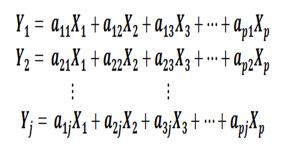
\includegraphics[]{Capture4.JPG}
\centering
\end{figure}

\end{comment}



\begin{comment}
\subsection{Network Time Protocol}

Sinkronisasi waktu jaringan mengacu pada penyimpangan batas waktu yang dilakukan oleh berbagai komunikasi atau komputer perangkat dalam jaringan dalam rentang yang cukup kecil\cite{ntp1}, sinkronisasi waktu pada jaringan dan server dapat dilakukan dengan berbagai metode, salah satunya adalah NTP. Keunggulan dari NTP memiliki akurasi tinggi serta dapat menggunakan berbagai alat sebagai referensi waktu seperti GPS, Time Code d.l.l. NTP bekerja dengan cara klien NTP memulai pertukaran permintaan waktu dengan server NTP. Sebagai hasil dari pertukaran ini, klien dapat menghitung penundaan tautan dan offset lokalnya, dan menyesuaikan jam lokal agar sesuai dengan jam di komputer server.

Dibandingkan dengan protokol lainnya untuk sinkronisasi waktu seperti SNTP (Simple Network Time Protocol), NTP dapat lebih andal karena dapat menerima input waktu dari berbagai sumber sedangkan SNTP hanya dapat menggunakan satu sumber input waktu, dari jam hardware atau jam interface jaringan. Namun, kedua protocol ini dapat bertukar informasi mengenai waktu sehingga lebih memudahkan dalam perancangan sistem.
\end{comment}

%\subsection{Distributed Denial of Service}

\subsection{Dataset}

Dataset yang akan digunakan adalah NSL KDD \texttt{(github.com/defcom17/NSL\_KDD)} karena dataset KDD lama sudah tidak diperbaharui lagi sejak 1999 sehingga sudah tidak relevan dengan gambaran serangn DDoS saat ini.
Data yang digunakan sendiri berjumlah 173.708 dengan koneksi bertipe normal sebanyak 90.502, dos sebanyak 62.621, probe sebanyak 16.366, r2l sebanyak 4.089, dan u2r sebanyak 130.

\subsection{Server}
\subsubsection{Operating System}

\textit{Operating System} yang akan digunakan adalah Linux OS dengan Ubuntu versi 18.04 karena fleksibilitas dari ubuntu dan dukungan dari komunitas yang banyak membuat ubuntu sesuai untuk dijadikan platform ubntuk percobaan.

\subsubsection{IDS (\textit{Intrusion Detection System})}
Snort adalah \textit{Network Intrusion Detection System} (NIDS) \textit{open source} yang mampu melakukan analisis lalu lintas jaringan secara \textit{real-time} dan paket logging pada jaringan. Snort juga dapat melakukan analisis protokol, pencarian / pencocokan konten, dan dapat digunakan untuk mendeteksi berbagai serangan dan probe, seperti buffer overflows, \textit{stealth port scans}, serangan CGI, probe SMB, percobaan SMB, dan banyak lagi.


\section{Pengujian}
%\subsection{Visualisasi Data}
Pengujian dilakukan dengan melakukan reduksi dimensi dataset menggunakan \textit{Principal Component Analysis} kemudian ditentukan beberapa fitur yang paling signifikan pada dataset. Reduksi data pada PCA ini mengunakan prinsip \textit{feature elimintaion} dengan tujuan untuk menghapus fitur-fitur yang dianggap tidak dibutuhkan untuk klasifikasi dan prediksi kemudian akan fokus kepada fitur-fitur yang dianggap berperan pada klasifikasi dan prediksi dataset.


\subsection{Training Dataset}

Melakukan reduksi dimensi data dengan \textit{Principal Component Analysis} kemudian dipilih fitur yang paling berpengaruh terhadap data sehingga didapatkan 5 fitur, 18 fitur dan kemudian dibandingkan dengan data asli dengan 41 fitur. \textit{Tools} yang digunakan adalah Python 3 dengan sklearn sebagai library utama. 
Langkah pertama adalah dengan memilih 41 data kemudian mereduksi dengan PCA. Kemudian dilihat rata-rata dari setiap fitur dan diambil yang positif.

Percobaan dilakukan menggunakan Python3 pada Google Colab dengan GPU aktif serta scikit-learn sebagai library utama. Data tes berjumlah 30\% dari total jumlah data (173708) dan data \textit{training} berjumlah 30\% dari total data dengan \textit{hidden layer} 100 (default sklearn). Data tes asli sendiri berjumlah 12\% (22543) dari keseluruhan data, tetapi data tes yang digunakan adalah 30\% dari total karena memiliki akurasi yang lebih baik daripada data tes asli.

Pada data sendiri ada modifikasi data dengan merubah beberapa data yang bertipe string menjadi integer namun karena data pada fitur adalah bersifat unik (tidak ada yang sama antara satu fitur dengan lainnya) maka perubahan data tersebut tidak mempengaruhi hasil.


Percobaan pertama adalah dengan \textit{running} algoritma terhadap dataset tanpa melakukan penyerdahanaan label (target), sebelum penyerdahanaan label berjumlah 39 setelah penyerdahaan berjumlah 5, kemudian didapatkanlah hasil waktu \textit{training} dan akurasinya.




\subsection{Principal Component Analysis}

Tujuan penggunaan PCA adalah untuk mereduksi dimensi dari data sehingga dapat data dapat diseleksi lebih cepat untuk menentukan fitur-fitur yang signifikan untuk menentukan klasifikasi algoritma terhadap data. Dengan menggunakan PCA, data asli yang semula 41 fitur akan direduksi menjadi 18 fitur paling berperngaruh terhadap data kemudian akan dibandingkan dengan 41 fitur keseleruhan tingkat akurasinya serta waktu trainingnya.

\begin{comment}
\subsubsection{Visualisasi PCA}
\end{comment}

\begin{comment}

\subsection{Rule Snort}
\textit{Rule} yang digunakan pada percobaan ini adalah Community Rule yang dapat diperoleh melalui \textit{website} snort \texttt{https://www.snort.org/downloads/community/snort3-community-rules.tar.gz}

\end{comment}



\begin{comment}
\subsubsection{41 Fitur}
Akurasi 97,88287\% dengan waktu training 444 detik.
\subsubsection{18 Fitur}
Akurasi 96,289512\% dengan waktu training 206 detik.

\begin{figure}[h]
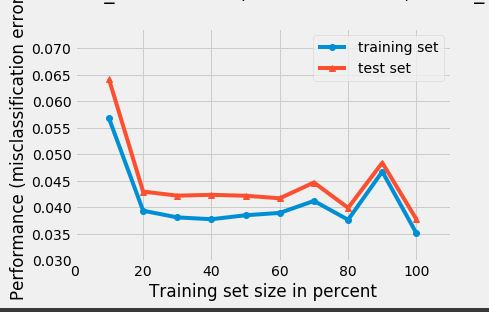
\includegraphics[scale=0.5]{18 fitur.JPG}
\centering
\caption{Learning Rate}
\end{figure}

\subsubsection{5 Fitur}
Akurasi yang dihasilkan 89.746005\% dengan waktu training 411 detik.
Terjadi anomali pada percobaan kali ini karena waktu training pada 18 fitur sudah menurun seperti yang diharapkan tetapi kembali lagi pada percobaan dengan 5 fitur yang paling signifikan. Awalnya diharapkan waktu \textit{training} menurun hingga menyentuh angka 150 detik tetapi terjadi anomali ini.
\end{comment}

\subsection{Hasil}
\FloatBarrier
\begin{table}[h]
\begin{tabular}{|r|r|r|}
\hline
\multicolumn{1}{|l|}{Fitur} & \multicolumn{1}{l|}{Waktu Training (s)} & \multicolumn{1}{l|}{Akurasi} \\  \hline
18                          & 206                                     & 96,28\%                      \\ \hline
41                          & 444                                     & 96,88\%                      \\ \hline
\end{tabular}
\centering
\caption{Hasil akurasi \textit{training dataset}}
\end{table}
\FloatBarrier

\begin{comment}

\FloatBarrier
\begin{table}[h]
\begin{tabular}{|r|r|r|}
\hline
\multicolumn{1}{|l|}{Fitur} & \multicolumn{1}{l|}{Waktu Training (s)} & \multicolumn{1}{l|}{Akurasi} \\  \hline
18                          & 178                                     & 96,13\%                      \\ \hline
41                          & 250                                     & 96,68\%                      \\ \hline
\end{tabular}
\centering
\caption{Hasil \textit{training} dengan label yang disederhanakan}
\end{table}
\FloatBarrier

\end{comment}



\FloatBarrier
\begin{table}[h]
\begin{tabular}{|r|r|r|}
\hline
\multicolumn{1}{|l|}{Fitur} & \multicolumn{1}{l|}{Waktu Training (s)} & \multicolumn{1}{l|}{Akurasi} \\  \hline
18                          & 180                                     & 99,40\%                      \\ \hline
41                          & 130                                     & 99.68\%                      \\ \hline
\end{tabular}
\centering
\caption{akurasi \textit{training} dengan PCA}
\end{table}
\FloatBarrier


\FloatBarrier
\begin{table}[]
\begin{tabular}{|l|r|r|}
\hline
Jumlah Atribut & \multicolumn{1}{l|}{Waktu Training (s)} & \multicolumn{1}{l|}{Akurasi (\%)} \\ \hline
1              & 41.48                                   & 94.62                             \\ \hline
2              & 119.93                                  & 95.29                             \\ \hline
3              & 101.35                                  & 97.02                             \\ \hline
4              & 126.14                                  & 98.46                             \\ \hline
5              & 119.01                                  & 98.84                             \\ \hline
6              & 119.96                                  & 99.12                             \\ \hline
7              & 98.54                                   & 99.29                             \\ \hline
8              & 94.82                                   & 99.27                             \\ \hline
9              & 83.10                                   & 99.41                             \\ \hline
10             & 60.98                                   & 99.46                             \\ \hline
11             & 63.59                                   & 99.51                             \\ \hline
12             & 85.71                                   & 99.54                             \\ \hline
13             & 74.78                                   & 99.61                             \\ \hline
14             & 40.74                                   & 99.59                             \\ \hline
15             & 67.76                                   & 99.60                             \\ \hline
16             & 51.68                                   & 99.61                             \\ \hline
17             & 77.16                                   & 99.69                             \\ \hline
18             & 54.40                                   & 99.67                             \\ \hline
19             & 41.38                                   & 99.61                             \\ \hline
20             & 57.01                                   & 99.71                             \\ \hline
21             & 55.94                                   & 99.69                             \\ \hline
22             & 50.32                                   & 99.71                             \\ \hline
23             & 63.76                                   & 99.54                             \\ \hline
24             & 60.18                                   & 99.72                             \\ \hline
25             & 55.38                                   & 99.71                             \\ \hline
26             & 60.52                                   & 99.73                             \\ \hline
27             & 36.56                                   & 99.68                             \\ \hline
28             & 57.54                                   & 99.73                             \\ \hline
29             & 59.04                                   & 99.85                             \\ \hline
30             & 32.08                                   & 99.88                             \\ \hline
31             & 30.90                                   & 99.85                             \\ \hline
32             & 35.28                                   & 99.84                             \\ \hline
33             & 36.92                                   & 99.86                             \\ \hline
34             & 41.70                                   & 99.85                             \\ \hline
35             & 36.98                                   & 99.84                             \\ \hline
36             & 47.97                                   & 99.85                             \\ \hline
37             & 29.87                                   & 99.86                             \\ \hline
38             & 41.33                                   & 99.86                             \\ \hline
39             & 31.98                                   & 99.87                             \\ \hline
40             & 38.64                                   & 99.86                             \\ \hline
41             & 31.48                                   & 99.86                             \\ \hline
\end{tabular}
\centering
\caption{akurasi dan waktu training keseluruhan}
\end{table}

\FloatBarrier



\section{Evaluasi}
Dari hasil percobaan ditemukan bahwa data yang diperoleh dari reduksi data yakni 18 fitur memiliki akurasi yang hampir mendekati akurasi dari 41 fitur.
Sedangkan percobaan dengan 18 fitur paling signifikan menghasilkan akurasi data yang hampir sama dengan waktu \textit{training} yang menurun hingga 64\%. 

Namun ketika label pada dataset disederhanakan dari sebelumnya 39 label menjadi 5 label yakni normal, dos, probe, r2l, dan u2r waktu training menjadi lebih cepat hingga 44\% dari sebelumnya. Sedangkan hasil training dengan PCA berhasil menurunkan waktu \textit{training} secara keseluruhan bahkan dengan 41 fitur memilik waktu \textit{training} yang paling cepat dengan akurasi 99\%. Waktu \textit{training} menjadi lebih cepat karena PCA langsung diterapkan pada data dan label juga disederhanakan.

Dengan demikian percobaan yang dilakukan berhasil menurunkan waktu training dan menaikan akurasi dari klasifikasi data.

\section{Kesimpulan}
Dengan mereduksi dimensi dataset yang berjumlah 41, waktu komputasi untuk training menjadi berkurang hinga 64\% sehingga mempercepat waktu deteksi, namun mengakibatkan akurasi deteksi sedikit menurun. Metode yang diusulkan berhasil menurunkan waktu training data. Namun ketika label disederhanakan waktu untuk \textit{training} menurun untuk kesemuanya sehingga tujuan untuk mempercepat \textit{training} data berhasil dicapai. PCA sebagai algoritma untuk mereduksi dimensi dapat bekerja seperti yang diharapkan dan mampu meraih akurasi yang sangat baik, namun studi lebih lanjut terkait algoritma dan cara memperlakukan data (\textit{treatment}) tetap diperlukan, studi lebih lanjut dengan menggunakan paradigma \textit{Deep Learning} juga dapat dikembangkan pada studi ini.

\section{Saran}
Studi lebih lanjut dengan \textit{treatment} data yang lebih baik dibutuhkan sehingga akurasi yang didapatkan lebih baik, selain itu penggunaan algoritma yang lebih baik juga memungkinkan akurasi deteksi dapat ditingkatkan. Kesalahan \textit{treatment} data yang dilakukan selama percobaan memungkinkan waktu \textit{training} menjadi tidak berbeda jauh pada percobaan 5 fitur. Sehingga pengembangan lebih jauh terhadap PCA dan aNN untuk klasifikasi serta deteksi DoS masih memungkinkan sehingga mencapai akurasi yang lebih baik dan waktu deteksi yang lebih cepat.


\bibliographystyle{abbrv}
\bibliography{references}% silakan ubah pada file paper.tex

\end{document}
